\documentclass[a4paper,12pt]{book}
\usepackage[utf8]{inputenc}
\title{}
\author{Rachel Morris}
\date{\today}

\usepackage{rachwidgets}
\usepackage{fancyhdr}
\usepackage{lastpage}
\usepackage{dirtree}
\usepackage{boxedminipage}
\usepackage{colortbl} % cell bg colors

\setcounter{chapter}{4}
\setcounter{section}{3}
\newcommand{\laChapter}{4.4 Properties of Relations\ }
\newcounter{question}

\newcommand{\laClass}{CS 210\ }
\newcommand{\laSemester}{Fall 2017\ }

\pagestyle{fancy}
\fancyhf{}
\lhead{\laClass \laSemester}
\chead{}
\rhead{Ch \laChapter}
\rfoot{\thepage\ of \pageref{LastPage}}
\lfoot{\scriptsize Compiled by Rachel Morris, last updated \today}

\renewcommand{\headrulewidth}{2pt}
\renewcommand{\footrulewidth}{1pt}

\begin{document}

    \toggletrue{answerkey}
    \togglefalse{answerkey}

    %------------------------------------------------------------------%
    %- Exercise Begin -------------------------------------------------%
    %------------------------------------------------------------------%

    \section{Properties of Relations}

    \subsection{Relations}

    \notonkey{
        \begin{introNOHEAD}{}
            \textbf{Relations:} A Relation is a way to relate two sets
            of data together. The two sets are the Domain and Codomain,
            and there is a Rule that associates them together.

            \begin{wrapfigure}{r}{0.4\textwidth}
                \tab[0.5cm]
                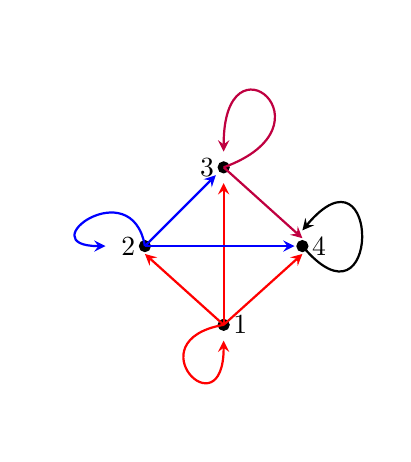
\begin{tikzpicture}[arrow/.style = {thick,-stealth}]
                    \filldraw (0,1) circle (2pt) node[left] {2};
                    \filldraw (2,1) circle (2pt) node[right] {4};
                    \filldraw (1,0) circle (2pt) node[right] {1};
                    \filldraw (1,2) circle (2pt) node[left] {3};

                    \draw[arrow,red] (1,0) -- (2,0.9);
                    \draw[arrow,red] (1,0) -- (0,0.9);
                    \draw[arrow,red] (1,0) -- (1,1.8);
                    \draw[arrow,red] (1,0)
                        to [out=-170, in=-90, looseness=15] (1,-0.2);

                    \draw[arrow,blue] (0,1) -- (0.9,1.9);
                    \draw[arrow,blue] (0,1) -- (1.9,1);
                    \draw[arrow,blue] (0,1)
                        to [out=100, in=180, looseness=5] (-0.5, 1);

                    \draw[arrow,purple] (1,2) -- (2,1.1);
                    \draw[arrow,purple] (1,2)
                        to [out=20, in=90, looseness=20] (1,2.2);

                    \draw[arrow,black] (2,1)
                        to [out=-50, in=50, looseness=20] (2,1.2);
                \end{tikzpicture}
            \end{wrapfigure}

            \subparagraph{Example:}
            $R : \{1,2,3\} \to \{1,2,3\}$; \\

            The relation $R$ has a domain of $\{1,2,3\}$ and a
            codomain of $\{1, 2, 3\}$. \\

            The rule is: $(x,y) \in R$ if $x \leq y$;
            so there is a relation (an arrow) from $x$ to $y$ if
            $x$ is less than or equal to $y$. 1 points to 1, 2, 3, and 4,
            2 points to 2, 3, and 4, and 3 points to 3 and 4, and 4 only points to itself.
        \end{introNOHEAD}
    }{}


    % -------------------------------------------------------------%
    % - QUESTION --------------------------------------------------%
    % -------------------------------------------------------------%
    \stepcounter{question}
    \begin{questionNOGRADE}{\thequestion}

        Draw the arrows for the following relations:

        \begin{center}
            \begin{tikzpicture}[arrow/.style = {thick,-stealth}]
                \node [below] at (0,4) {$R$};

                    \filldraw (0,1) circle (2pt) node[left] {2};
                    \filldraw (2,1) circle (2pt) node[right] {4};
                    \filldraw (1,0) circle (2pt) node[right] {1};
                    \filldraw (1,2) circle (2pt) node[left] {3};

                    \solution{
                        \draw[arrow] (1,0) -- (0,0.9);
                        \draw[arrow] (0,1) -- (1,1.9);
                        \draw[arrow] (1,2) -- (2,1.1);
                    }{}

                \node [below] at (5,4) {$S$};
                    \filldraw (7,2) circle (2pt) node[below] {1};
                    \filldraw (5,0) circle (2pt) node[left] {2};
                    \filldraw (7,0) circle (2pt) node[right] {3};
                    \filldraw (5,2) circle (2pt) node[left] {4};

                    \solution{
                        \draw[arrow] (5,0) -- (6.9,0);
                        \draw[arrow] (5,0) -- (5,1.9);
                        \draw[arrow] (7,0) -- (5.2,2);

                        \draw[arrow] (7,2)
                            to [out=0, in=90, looseness=15] (7,2.2);
                    }{}

            \end{tikzpicture}
        \end{center}

        ~\\

        Set $A$ is $A = \{1, 2, 3, 4\}$.

        Relation $R$: $R : A \to A$, with the rule:
            $\{ (1,2), (2,3), (3,4) \}$

        Relation $S$: $S : A \to A$, with the rule:
            $\{ (1,1), (2,3), (2,4), (3,4) \}$

    \end{questionNOGRADE}

    \notonkey{ \newpage }{ \hrulefill }

    \notonkey{
        \begin{introNOHEAD}{}
            \paragraph{Properties of Binary Relations} ~\\
            Let $R$ be a binary relation on set $A$.

            \subparagraph{Reflexive:} $R$ is said to be reflexive if
            $(a,a) \in R$ for all $a \in A$. In terms of the arrow
            diagram, this means that \textbf{every node has a loop}.

            \subparagraph{Irreflexive:} A relation $R$ on set $A$ is irreflexive
            if, for all $a \in A$, $(a,a) \not\in R$. On the arrow diagram,
            this means \textbf{there are no loops.}

            \subparagraph{Symmetric:} $R$ is called symmetric if
            for all $a,b \in A$, if $a \neq b$ and $(a,b) \in R$,
            then $(b,a) \in R$. In terms of the arrow diagram, this
            means that \textbf{every arrow goes in both directions}.

            \subparagraph{Antisymmetric:} $R$ is called antisymmetric if
            for all $a,b \in A$, if $a \neq b$ and $(a,b) \in R$,
            then $(b,a) \not\in R$. In terms of the arrow diagram, this
            means that \textbf{arrows only go in one direction}.

            \subparagraph{Transitive:} $R$ is transitive if, whenever
            $(a,b) \in R$ and $(b,c) \in R$, it must also be the case
            that $(a,c) \in R$. In terms of the arrow diagram, this
            means that \textbf{whenever you can follow two arrows
            to get from node $a$ to node $c$, you can also get there
            along a single arrow}.
            \footnote{Discrete Mathematics, Ensley and Crawley}

            ~\\
            Note that relations can be Reflexive, Irreflexive, or Neither,
            as well as Symmetric, Antisymmetric, or Neither.
        \end{introNOHEAD}
    }{}

    \newpage

    % -------------------------------------------------------------%
    % - QUESTION --------------------------------------------------%
    % -------------------------------------------------------------%
    \stepcounter{question}
    \begin{questionNOGRADE}{\thequestion}

        ~\\
        Complete the arrow diagram for the relation on
        \small
        $A$ = \{1, 2, 3, 4, 5, 6, 7, 8\}.
        \normalsize
        Also identify the properties of each. Give reasons why the relation is
        transitive, intransitive, neither, symmetric, antisymmetric, neither, and/or
        reflexive.

        ~\\
        $ R_{1} $ = \{    (1,1), (1,2), (1,4), (1,8), \tab
                        (2,2), (2,4), (2,8), \tab
                        (3,3), (3,6), \\ \tab[1.3cm]
                        (4,4), (4,8) \tab
                        (5,5), \tab (6,6), \tab (7,7), \tab (8,8)
                 \}

        \solution{
            \begin{center}
                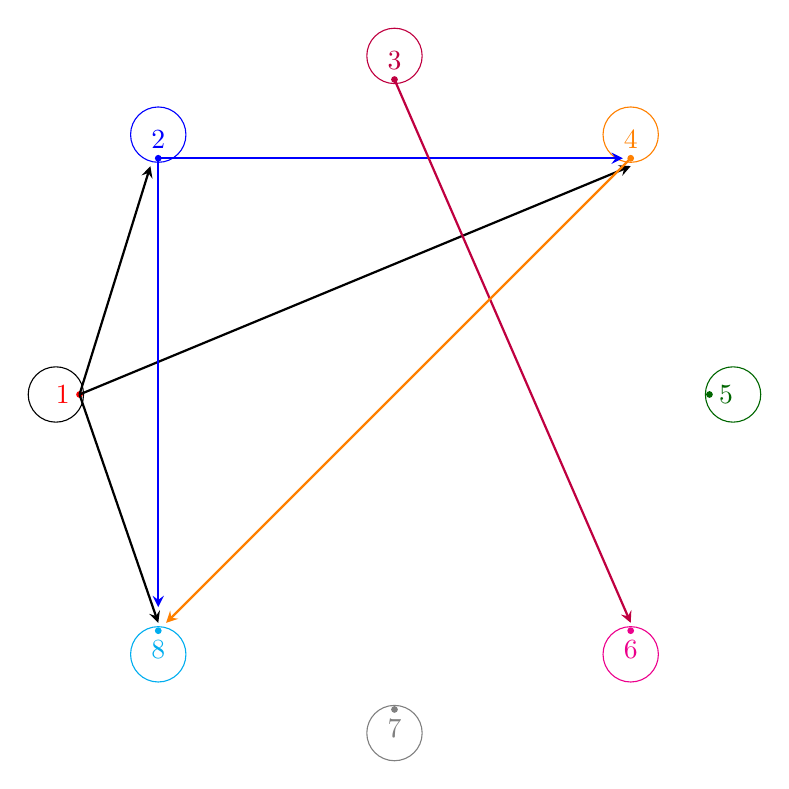
\begin{tikzpicture}[arrow/.style = {thick,-stealth}]
                    \filldraw[red]              (-4,0)          circle (1pt) node[left]  {1};
                    \filldraw[blue]             (-3,3)          circle (1pt) node[above] {2};
                    \filldraw[purple]           (0,4)           circle (1pt) node[above] {3};
                    \filldraw[orange]           (3,3)           circle (1pt) node[above] {4};
                    \filldraw[black!60!green]   (4,0)           circle (1pt) node[right] {5};
                    \filldraw[magenta]          (3,-3)          circle (1pt) node[below] {6};
                    \filldraw[gray]             (0,-4)          circle (1pt) node[below] {7};
                    \filldraw[cyan]             (-3,-3)         circle (1pt) node[below] {8};

                    \draw (-4.3, 0) circle (10pt);
                    \draw[blue] (-3, 3.3) circle (10pt);
                    \draw[purple] (0, 4.3) circle (10pt);
                    \draw[orange] (3, 3.3) circle (10pt);
                    \draw[black!60!green] (4.3, 0) circle (10pt);
                    \draw[magenta] (3,-3.3) circle (10pt);
                    \draw[gray] (0,-4.3) circle (10pt);
                    \draw[cyan] (-3,-3.3) circle (10pt);

                    \draw[arrow] (-4,0) -- (-3.1,2.9);
                    \draw[arrow] (-4,0) -- (3, 2.9);
                    \draw[arrow] (-4,0) -- (-3, -2.9);

                    \draw[blue,arrow] (-3,3) -- (2.9, 3);
                    \draw[blue,arrow] (-3,3) -- (-3, -2.7);

                    \draw[purple,arrow] (0,4) -- (3,-2.9);

                    \draw[orange,arrow] (3,3) -- (-2.9,-2.9);

                \end{tikzpicture}
            \end{center}
        }{
            \begin{center}
                \begin{tikzpicture}
                    \filldraw (-2,0)        circle (1pt) node[left] {1};
                    \filldraw (-1.5,1.5)    circle (1pt) node[above] {2};
                    \filldraw (0,2)         circle (1pt) node[above] {3};
                    \filldraw (1.5,1.5)     circle (1pt) node[above] {4};
                    \filldraw (2,0)         circle (1pt) node[right] {5};
                    \filldraw (1.5,-1.5)    circle (1pt) node[below] {6};
                    \filldraw (0,-2)        circle (1pt) node[below] {7};
                    \filldraw (-1.5,-1.5)   circle (1pt) node[below] {8};
                \end{tikzpicture}
            \end{center}
        }

        \vspace{1cm}

        \Square\ Reflexive? \tab
        \Square\ Irreflexive? \tab
        \Square\ Neither? \tab Why?
        \solution{ ~\\
            It is reflexive - All elements of $A$ point back to itself (every node has a loop).
        }{ \vspace{2.5cm} }

        \Square\ Symmetric? \tab
        \Square\ Antisymmetric? \tab
        \Square\ Neither? \tab Why?
        \solution{ ~\\
            It is antisymmetric - No arrows go in both directions.
        }{ \vspace{2.5cm} }

        \Square\ Transitive? \tab Why?
        \solution{ ~\\
            It is transitive - All two-arrow paths also have a direct arrow between the endpoints.
        }{ \vspace{2.5cm} }

    \end{questionNOGRADE}


    \newpage


    % -------------------------------------------------------------%
    % - QUESTION --------------------------------------------------%
    % -------------------------------------------------------------%
    \stepcounter{question}
    \begin{questionNOGRADE}{\thequestion}

        ~\\
        Complete the arrow diagram for the relation on
        \small
        $A$ = \{1, 2, 3, 4, 5, 6, 7, 8\}.
        \normalsize
        Also identify the properties of each. Give reasons why the relation is
        transitive, intransitive, neither, symmetric, antisymmetric, neither, and/or
        reflexive.

        FIXME: KEY SHOULD HAVE LOOPS

        ~\\
        $ R_{2} $ = \{  (1,1), (1,3), (1,5), (1,7) \tab
                        (2,2), (2,4), (2,8), \\ \tab[1.3cm]
                        (3,3), (3,5), (3,7), \tab
                        (4,2), (4,4), (4,8), \tab
                        (5,3), (5,7), \\ \tab[1.3cm]
                        (6,6), (6,8), \tab
                        (8,2), (8,4), (8,8)
                 \}

        \solution{
            \begin{center}
                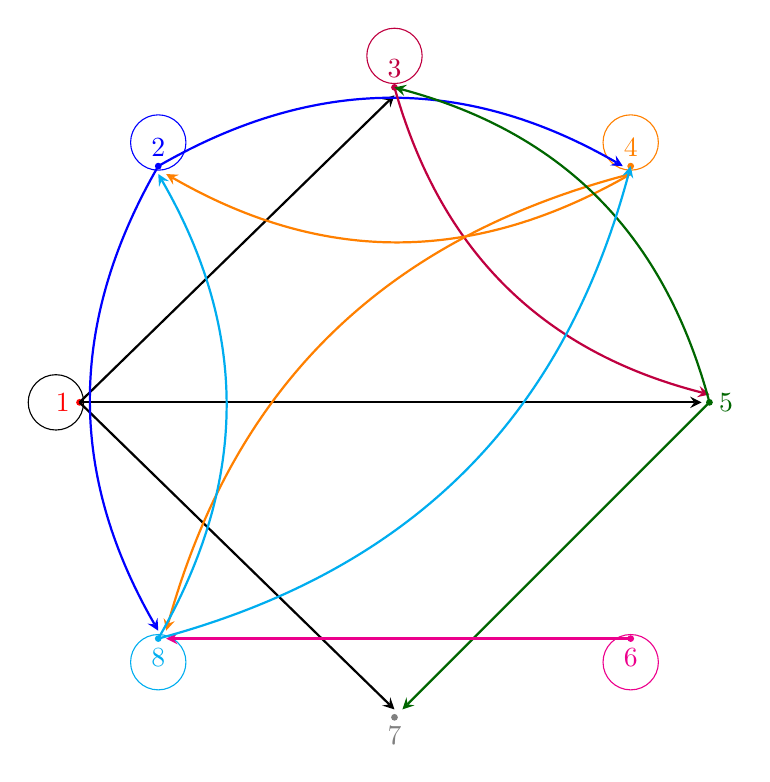
\begin{tikzpicture}[arrow/.style = {thick,-stealth}]
                    \filldraw[red]              (-4,0)        circle (1pt) node[left]  {1};
                    \filldraw[blue]             (-3,3)    circle (1pt) node[above] {2};
                    \filldraw[purple]           (0,4)         circle (1pt) node[above] {3};
                    \filldraw[orange]           (3,3)     circle (1pt) node[above] {4};
                    \filldraw[black!60!green]   (4,0)         circle (1pt) node[right] {5};
                    \filldraw[magenta]          (3,-3)    circle (1pt) node[below] {6};
                    \filldraw[gray]             (0,-4)        circle (1pt) node[below] {7};
                    \filldraw[cyan]             (-3,-3)   circle (1pt) node[below] {8};

                    % loops
                    \draw (-4.3, 0) circle (10pt);
                    \draw[blue] (-3, 3.3) circle (10pt);
                    \draw[purple] (0, 4.4) circle (10pt);
                    \draw[orange] (3, 3.3) circle (10pt);
                    \draw[magenta] (3,-3.3) circle (10pt);
                    \draw[cyan] (-3,-3.3) circle (10pt);

                    % 1
                    \draw[arrow] (-4,0) -- (3.9, 0);
                    \draw[arrow] (-4,0) -- (0,3.9);
                    \draw[arrow] (-4,0) -- (0, -3.9);

                    % 2
                    \draw[blue,arrow] (-3,3) to[bend left] (2.9, 3);
                    \draw[blue,arrow] (-3,3) to[bend right] (-3, -2.9);

                    % 3
                    \draw[purple,arrow] (0,4) to[bend right] (4,0.1);

                    % 4
                    \draw[orange,arrow] (3,2.9) to[bend left] (-2.9, 2.9);
                    \draw[orange,arrow] (3,2.9) to[bend right] (-2.9, -2.9);

                    % 5
                    \draw[black!60!green,arrow] (4,0) to[bend right] (0,4);
                    \draw[black!60!green,arrow] (4,0) -- (0.1,-3.9);

                    % 6
                    \draw[magenta,arrow] (3,-3) -- (-2.9, -3);

                    % 7
                    \draw[cyan,arrow] (-3,-3) to[bend right] (-3,2.9);
                    \draw[cyan,arrow] (-3,-3) to[bend right] (3, 3);

                \end{tikzpicture}
            \end{center}
        }{
            \begin{center}
                \begin{tikzpicture}
                    \filldraw (-2,0)        circle (1pt) node[left] {1};
                    \filldraw (-1.5,1.5)    circle (1pt) node[above] {2};
                    \filldraw (0,2)         circle (1pt) node[above] {3};
                    \filldraw (1.5,1.5)     circle (1pt) node[above] {4};
                    \filldraw (2,0)         circle (1pt) node[right] {5};
                    \filldraw (1.5,-1.5)    circle (1pt) node[below] {6};
                    \filldraw (0,-2)        circle (1pt) node[below] {7};
                    \filldraw (-1.5,-1.5)   circle (1pt) node[below] {8};
                \end{tikzpicture}
            \end{center}
        }

        \vspace{1cm}

        \Square\ Reflexive? \tab
        \Square\ Irreflexive? \tab
        \Square\ Neither? \tab Why?
        \solution{ ~\\
            It is neither -- there are some loops, but not on all (reflexive)
                and not on none (irreflexive).
        }{ \vspace{2.5cm} }

        \Square\ Symmetric? \tab
        \Square\ Antisymmetric? \tab
        \Square\ Neither? \tab Why?
        \solution{ ~\\
            It is neither - some arrows go in both directions, but not all (symmetric),
                and not none (antisymmetric). e.g., (2,8) and (8,2) exist.
        }{ \vspace{2.5cm} }

        \Square\ Transitive? \tab Why?
        \solution{ ~\\
            It is NOT transitive: 6 goes to 8, and 8 goes to other places,
                but 6 doesn't go to other locations.
        }{ \vspace{2.5cm} }

    \end{questionNOGRADE}

\newpage

    \begin{intro}{Recap}
        \begin{itemize}
            \item   \textbf{Reflexive:}         $(a,a) \in R$ for all $a \in A$
            \item   \textbf{Irreflexive:}       $(a,a) \not\in R$ for all $a \in A$
            \item   \textbf{Antisymmetric:}     for all $a,b \in A$, if $a \neq b$ and $(a,b) \in R$, \\ then $(b,a) \not\in R$
            \item   \textbf{Transitive:}        if $(a,b) \in R$ and $(b,c) \in R$ then $(a,c) \in R$
        \end{itemize}
    \end{intro}

    % -------------------------------------------------------------%
    % - QUESTION --------------------------------------------------%
    % -------------------------------------------------------------%
    \stepcounter{question}
    \begin{questionNOGRADE}{\thequestion}

        Given the relation, $R_{1} = \{ (a,b) \in \mathbb{Z} \times \mathbb{Z} : a + b$ is even$\}$.

        \begin{itemize}
            \item[a.]   This relation is \textbf{reflexive}. Find an example to illustrate why.
                \begin{hint}{\ }
                    $a$ and $b$ are both in the set of integers. We are checking to see if the
                    result of $(a,a)$ is always in the relation $R_{1}$... so,
                    if you plug in $(a,a)$ into the relation, is the output still ``is even"?
                \end{hint}

                \solution{
                    Since $a + a = 2a$ is always even, we know that $(a,a) \in R_{1}$ for all $a \in \mathbb{Z}$.
                    Hence, $R_{1}$ is reflexive (and not irreflexive).
                }{\vspace{2cm}}

            \item[b.]   This relation is \textbf{symmetric}. Find an example to illustrate why.
                \begin{hint}{\ }
                    Find some $(a,b)$ and $(b,a)$ that are both in the relation.
                    If you can, it's symmetric.
                \end{hint}

                \solution{
                    Since $(1,3) \in R_{1}$ and $(3,1) \in R_{1}$, $R_{1}$ is symmetric.
                }{\vspace{2cm}}
        \end{itemize}

    \end{questionNOGRADE}

\newpage

    \begin{wrapfigure}{r}{0.4\textwidth} 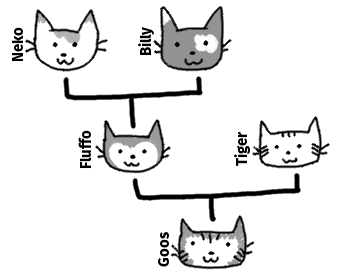
\includegraphics[height=5cm]{images/catfamily.png} \end{wrapfigure}
        
    % -------------------------------------------------------------%
    % - QUESTION --------------------------------------------------%
    % -------------------------------------------------------------%
    \stepcounter{question}
    \begin{questionNOGRADE}{\thequestion}

    
        Let $C$ be the set of all cats who have ever lived. For each of the
        following relations on the set $C$, decide if the given is
        reflexive irreflexive, transitive, or antisymmetric.
        Some of these can satisfy more than one property. Give
        explanations on how you decided each of these.
        

        \begin{itemize}
            \item[a.]   $R_{1} = \{ (a, b) \in C \times C : a$ is a child of $b \}$

                \begin{itemize}
                    \item   Reflexive - Is $(a,a) \in C$ for all $a$ valid?
                            \\ \textit{(For some cat $a$, $(a,a)$ means ``$a$ is a child of $a$''. Is this valid?)}
                            \solution{ no; a cat cannot be its own parent }{ \vspace{2cm} }

                    \item   Irreflexive - Is $(a,a) \not\in C$ for all $a$ valid?
                            \solution{ yes; a cat cannot be its own parent }{ \vspace{2cm} }

                    \item   Transitive - Is there some $(a,b) \in C$ and $(b,c) \in C$?
                            \footnote{Just assume a cat isn't going to mate with its child. $:|$}
                            \\ \textit{(For three cats $a$, $b$, and $c$, if $a$ is a chlid of $b$,
                            and $b$ is a child of $c$, can $a$ be a child of $c$?)}
                            \solution{
                                no; if ``Cat A" is a child of ``Cat B",
                                and ``Cat B" is a child of ``Cat C", then
                                ``Cat A" cannot also be a child of ``Cat C".
                            }{ \vspace{2cm} }

                    \item   Antisymmetric - Is $(a,b) \in C$ and $(b,a) \not\in C$ valid?
                            \\ \textit{For some cat $a$ and $b$, can both of the following be true? ``$a$ is a child of $b$, and $b$ is a child of $a$'')}
                            \solution{
                            yes; if ``Cat A" is a child of ``Cat B", then ``Cat B" cannot be a child of ``Cat A".
                            }{ \vspace{1cm} }
                \end{itemize}

        \newpage

            \item[b.]   $R_{2} = \{ (a, b) \in C \times C : a$ is a descendant of $b \}$

                \begin{itemize}
                    \item   Reflexive - Is $(a,a) \in C$ for all $a$ valid?
                            \solution{
                                no; same as above
                            }{ \vspace{3cm} }

                    \item   Irreflexive - Is $(a,a) \not\in C$ for all $a$ valid?
                            \solution{
                                yes; same as above
                            }{ \vspace{3cm} }

                    \item   Transitive - Is there some $(a,b) \in C$ and $(b,c) \in C$?
                            \solution{
                                yes; f ``Cat A" is a descendant of ``Cat B" and ``Cat B" is
                                a descendant of ``Cat C", then ``Cat A" is also a
                                descendant of ``Cat C".
                            }{ \vspace{3cm} }

                    \item   Antisymmetric - Is $(a,b) \in C$ and $(b,a) \not\in C$ valid?
                            \solution{
                            yes; same as above
                            }{ \vspace{3cm} }
                \end{itemize}
        \end{itemize}


    \end{questionNOGRADE}




\end{document}








